\documentclass{article}
\title{QC Functions User Manual}
\author{Chen Chun-Yu}
\textwidth=6.2in
\textheight=8.5in
\oddsidemargin=.1in
\evensidemargin=.1in
\headheight=-.3in
\usepackage{subfigure}

\usepackage{Sweave}
\begin{document}
\Sconcordance{concordance:QC_user_manual.tex:QC_user_manual.Rnw:%
1 10 1 1 0 102 1}

\maketitle
\tableofcontents
\newpage
\section{Introduction}
This manual shows you how to use the quality control functions and give an example for demonstration.
\section{Prerequest}
To make the functions run successfully, please ensure you have installed PLINK in previous.\\
After you installed PLINK, please copy it from defult folder and paste it to /usr/local/bin.
\\\\\verb@$ cp ~/Bin/plink /usr/local/bin@
\section{Caution}
Do not modify any content arbitrarily of ouput files generated from PLINK!
\section{QC Functions}
\subsection{Per-individual QC}
\begin{itemize}
    \item sex\_check(input.name, output.name) \\
    Place the name of your PLINK binary files(BED/BIM/FAM) at "input.name" argument, and give the output name at "output.name" argument.
    After the analysis, you will get a plot("sex\_distribution.pdf") which shows the distribution of individual's sex and a 
    "output.name\_sex\_problem.list" file which records individuals with discordant sex information. Defult homozygosity rates of identifying 
    individual as male is above 0.8, and recognizing as female is below 0.2.
    \item missing\_het\_ind(input.name, pop.list, output.name) \\
    You still need to give input and ouput names for the analysis. You also need to give a list of individuals with their populations at "pop.list" argument, 
    the example format shows below:\\
    \begin{table}[ht]
    \centering
    \begin{tabular}{lcr}
    \hline
    1 & TDC13 & Paiwan \\ 
    2 & TDC117 & Amis \\ 
    3 & TDC18 & Bunun \\ 
    4 & TDC129 & Amis \\
    5 & TDC49 & Amis \\
    6 & TDC497 & Puyuma \\
    \hline
    \end{tabular}
    \end{table}\\
    You will get a plot("imiss-vs-het.pdf") which shows the distribution of missingness and heterozygosity scores and a 
    "output.name\_miss\_het\_problem.list" file which records individuals do not pass criteria. Default cuttoffs of genotype failure rates 
    are equal or larger than 0.03 and heterozygosity rates deviate more or less 3 s.d. from the mean.
    \item IBD(input.name, output.name) \\
    You still need to give input and ouput names for the analysis. After the analysis, you will get a plot("IBD.pdf") which shows the propotion 
    of the different IBD between pairs of individuals. You will also get a "output.name\_ibd\_problem.list" that records the individuals do not 
    pass the criterion. Default value of IBD we intend to remove is higher than 0.1875.
    \item ind\_qc\_rm(input.name, output.name) \\
    After you finish the steps of per-individual QC, you can use ind\_qc\_rm function to output the list("output.name\_fail\_ind\_qc.txt") which contains 
    all the problem lists that are generated by previous QC steps. You can use following PLINK command to remove the individuals easily:\\
    \\\verb@plink --bfile your.PLINK.bfile --remove output.name_fail_ind_QC.txt --make-bed --out output.name@
\end{itemize}
\subsection{Per-SNP QC}
\begin{itemize}
    \item missing\_snp(input.name, output.name) \\
    You still need to give input and ouput names for the analysis. You will get a plot("snpmiss\_plot.pdf") which shows the distribution of 
    missing genotype rate and a threshold for extreme genotype failure rate. Default missing genotype rate threshold is equal to 0.03.
    \item hwe\_test(input.name, output.name) \\
    You still need to give input and ouput names for the analysis. You will get a plot("hwe\_p\_value.pdf") which shows the distribution of 
    Hardy-Weinberg Equilibrium test's p-value and a threshold for extreme high p-value. Default extreme p-value threshold is equal to 0.00001.
\end{itemize}
Two per-SNP QC steps show above are aim to show the distribution of missing genotype rate and Hardy-Weinberg Equilibrium test's p-value. If you want to 
further exclude those SNPs, please use following PLINK commands:\\
\\\verb@plink --bfile your.PLINK.bfile --maf 0.01 --geno 0.03 --hwe 0.00001 --make-bed --out output.name@
\newpage
\section{Example}
Here we give you an example of applying the functions we have illustrated. The example data is consists of 96 individuals and about 2.5 millions of SNPs.\\
\subsection{Per-individual QC}

\begin{figure}[h]
    \centering
    \subfigure[Distribution of individual's sex.]
    {
        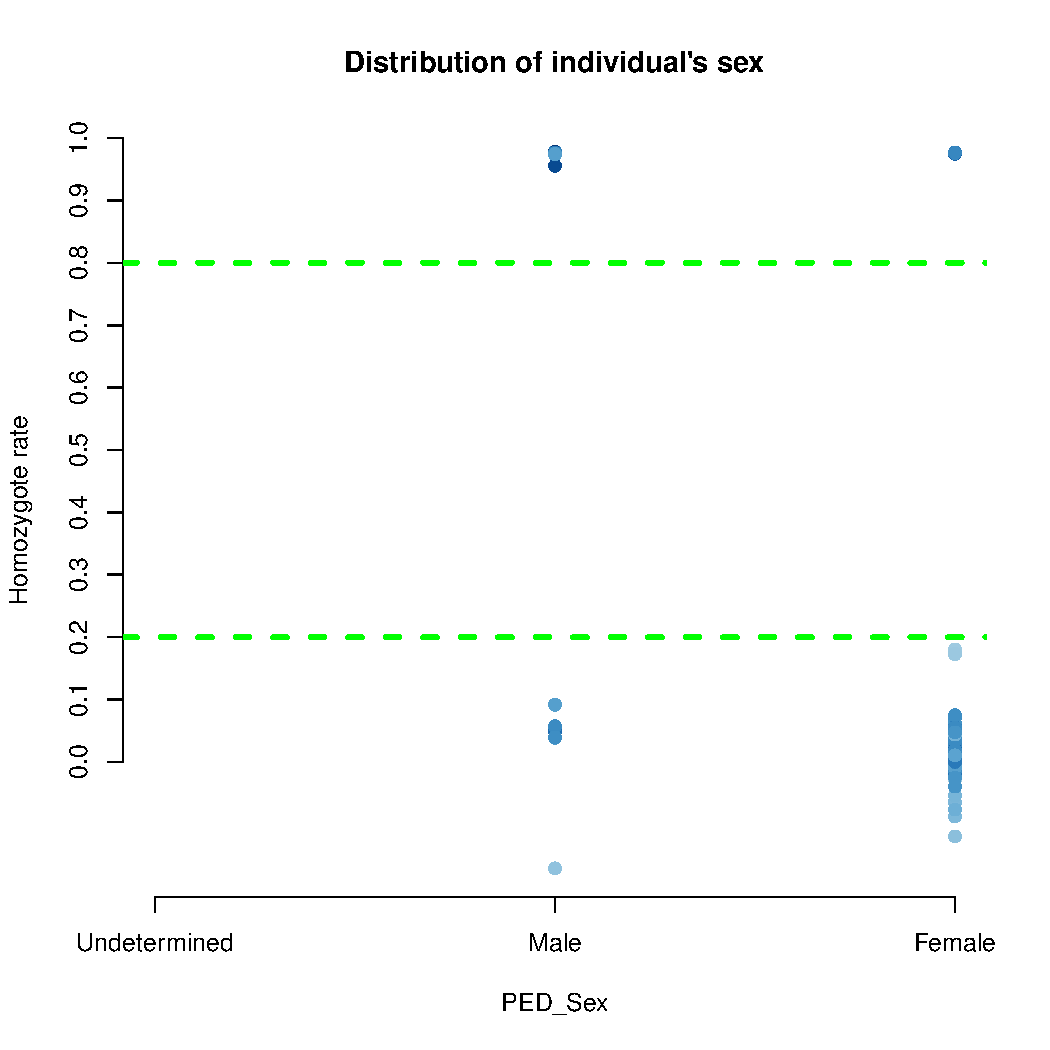
\includegraphics[width=2.8in]{/Users/chenchun-yu/Project/raw_data/sex_distribution.pdf}
    }
    \\
    \subfigure[Distribution of missingness and heterozygosity scores.]
    {
        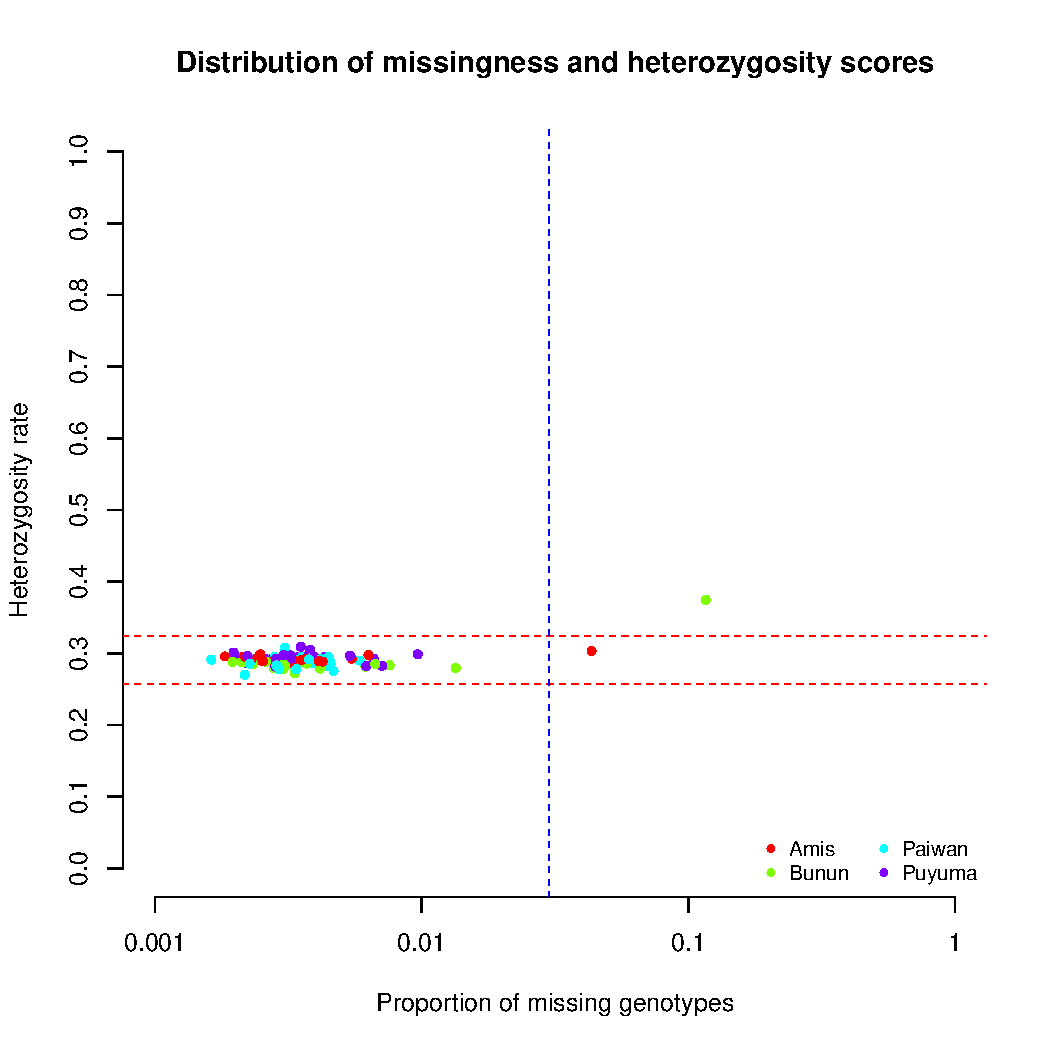
\includegraphics[width=2.8in]{/Users/chenchun-yu/Project/raw_data/imiss-vs-het.pdf}
    }
    \subfigure[Propotion of the different IBD]
    {
        \includegraphics[width=2.8in]{/Users/chenchun-yu/Project/raw_data/IBD.pdf}
    }
    \caption{Three analysis in per-individual QC.}
\end{figure}
\subsection{Per-SNP QC}
\begin{figure}[h]
    \centering
    \subfigure[Distribution of missing genotype rate.]
    {
        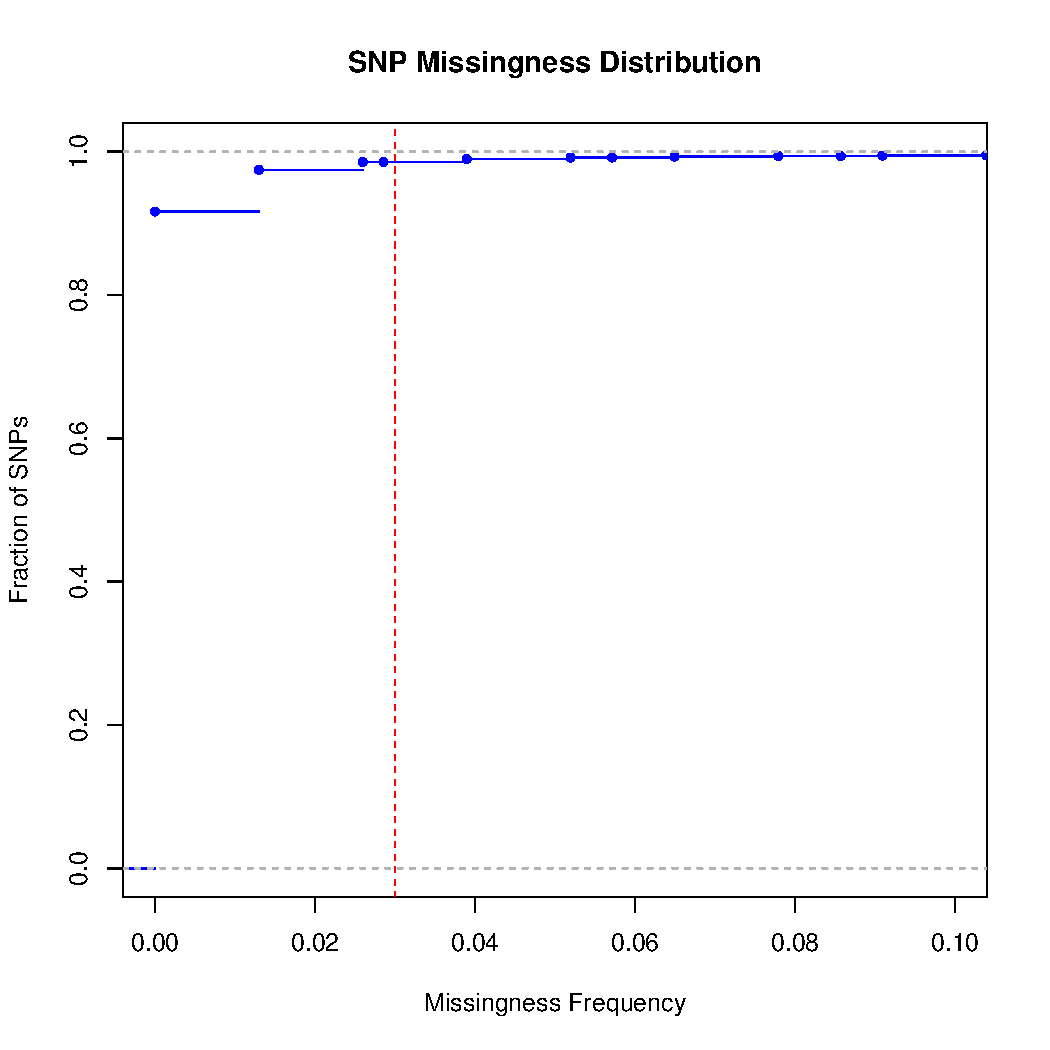
\includegraphics[width=2.8in]{/Users/chenchun-yu/Project/raw_data/snpmiss_plot.pdf}
    }
    \subfigure[Distribution of Hardy-Weinberg Equilibrium test's p-value.]
    {
        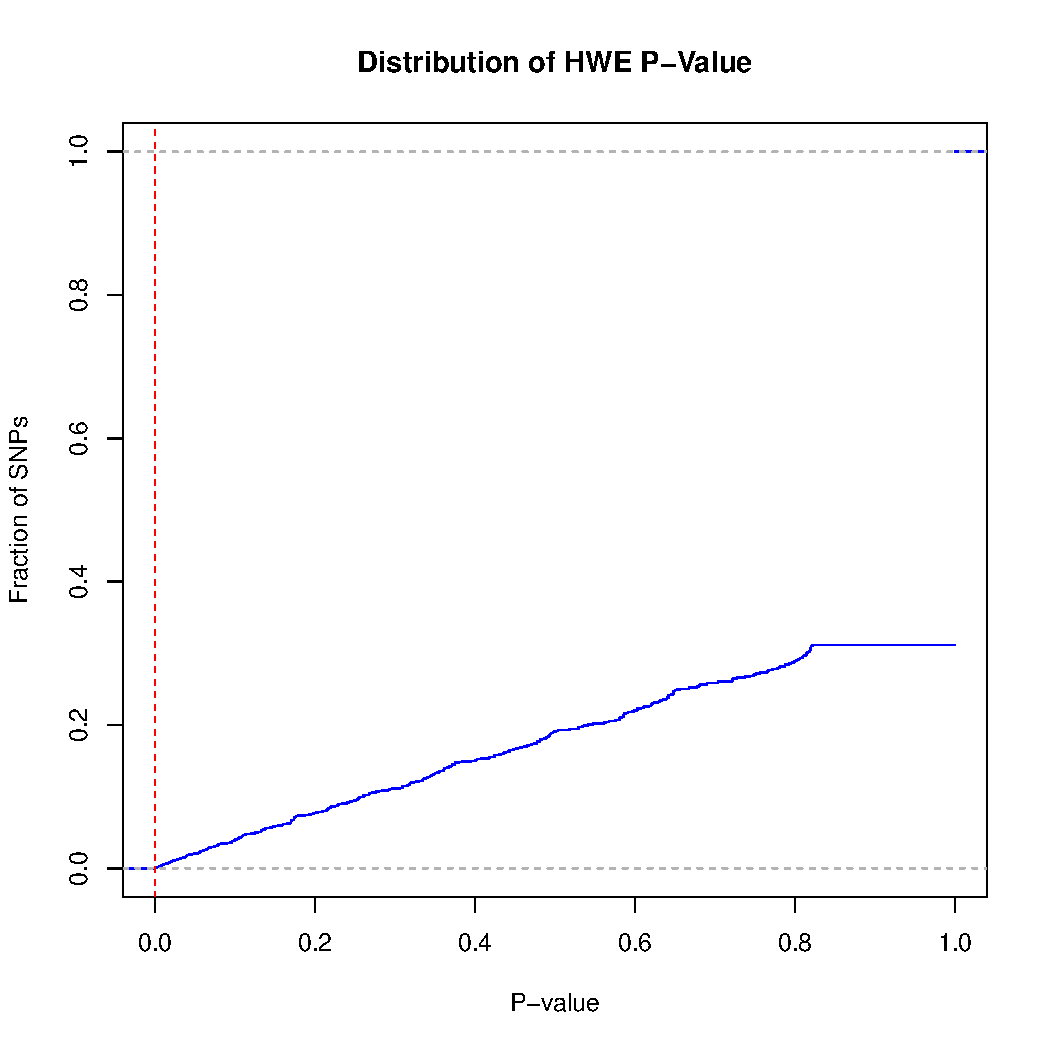
\includegraphics[width=2.8in]{/Users/chenchun-yu/Project/raw_data/hwe_p_value.pdf}
    }
    \caption{Two analysis in per-SNP QC.}
\end{figure}
\begin{thebibliography}{1}
\bibitem{notes} Anderson CA, Pettersson FH, Clarke GM, Cardon LR, Morris AP, Zondervan KT. {Data quality control in genetic case-control association studies. 
\em Nature protocols.} 2010;5(9):1564-1573. doi:10.1038/nprot.2010.116.
\bibitem{notes} Purcell S, Neale B, Todd-Brown K, et al. {PLINK: A Tool Set for Whole-Genome Association and Population-Based Linkage Analyses. 
\em American Journal of Human Genetics.} 2007;81(3):559-575.
\end{thebibliography}
\end{document}
